\chapter{Side project: Estimation of the variability in Cystic Fibrosis patients FEV1 lung function measurements} \label{sec:sideproject}

\section{Introduction}
The most commonly used lung function bio-marker, FEV1, contains a technical variability intrinsic to its measurement method. Producing a consistent "forced expiratory volume" indeed requires effort and focus, especially when this is performed individually as part of a home monitoring study like Project Breathe. This variability translates into a high noise, and thereby difficult interpretation of the measurements. Given the central role of FEV1 to evaluate patient's lung health in CF \cite{giron_2021}, it is important to have a criteria to distinguish signal from noise. The aim of this study is to provide an estimation of the day-to-day variability in FEV1 measurements performed at home by patients using a personal device. The variability is considered to be closely linked to the noise present in the time-series of measurements. Hence, a model is built to extract the noise and signal. The estimation of the variability in FEV1 corresponds to the noise component of the model. The data from Project Breathe until June 2021, described in appendix \ref{sec:appendixbreathe}, was used.

The code used to derive the results is documented \href{https://tristantreb.github.io/pdm/}{\textit{here}}.

\section{Material}
This section introduces the statistical material used to perform the hypothesis testing for equality of variance performed in \ref{sec:hptests}.

\subsection{Quantile-quantile plot}
Let X be a random variable and $F_X$ be its distribution function. The quantile function of X $F_X^{-1}$ is defined as:
\begin{equation}
    F_X^{-1} : (0,1) \longrightarrow \mathbb{R}, F_X^{-1}(\alpha) \longmapsto \inf \{ t \in \mathbb{R}: F_X(t) \geq \alpha \}
\end{equation}
The $\alpha$-quantile of X is the real number $q_\alpha = F_X^{-1}(\alpha)$.

A Q-Q plot is a graphical technique used to determine if two datasets come from populations with the same distribution. Given the quantile functions of two datasets, it plots the $\alpha$-quantiles of the first data set against the $\alpha$-quantiles of the second data set. If the distributions are similar, so are their quantiles for each $\alpha$, hence all the points will intercept the linear function $f : \mathbb{R} \longrightarrow \mathbb{R}, f(x) \mapsto x$. Many distributional aspects can simultaneously tested, such shifts in location or scale, changes in symmetry, presence of outliers. Since the quantile function is continuous, the Q-Q plot can be used with differently sized data sets. 

\subsection{Homoscedasticity tests} \label{sec:homoscedasticity}
Homoscedasticity tests are used to test if the variance of two populations are not equal. They has several formulations that are robust in different situations, mainly depending on the underlying distribution of the data sets available. The most traditional F-test as well as the Levene and Brown Forsythe tests are detailed.
Two concepts are important to define when it comes to choosing a test statistic. \textbf{Statistical power} is the availability to detect the alternative hypothesis when it is in fact true (true negative). \textbf{Statistical robustness} is the probability of false rejection of the null hypothesis caused by non-normality (false negative).

\subsubsection{F-test}
Let $\mathbf{X_1}$, $\mathbf{X_2}$ of size $N_1$, $N_2$, variance $s_1^2, s_2^2$ be two samples drawn from two normal distributions with respective variance $\sigma_1^2, \sigma_2^2$. The F hypothesis test is defined as:
\begin{center}
    $H_0 : \sigma_1^2 = \sigma_2^2,$
\end{center}
\begin{equation}
    H_a : 
    \begin{cases}
        \sigma_1^2 \neq \sigma_2^2, & \text{for a two-tailed test}\\
        \sigma_1^2 > \sigma_2^2, & \text{for a lower one-tailed test}\\
        \sigma_1^2 > \sigma_2^2, & \text{for an upper one-tailed test}\\
    \end{cases}
\end{equation}

The test stastistic F is degined as $F = \frac{s_1^2}{s_2^2 }$. The more the ratio deviates from 1, the stronger the evidence of unequal population variances.

Critical region: with the significance level $\alpha$, and degrees of freedom $v_1$, $v_2$ ($v$ = N-1), the alternative hypothesis is rejected if:
\begin{equation}
    \begin{cases}
        F < F_{1-\frac{\alpha}{2}, v_1, v_2} \text{ or } F > F_{\frac{\alpha}{2}, v_1, v_2}, & \text{for a two-tailed test}\\
        F > F_{\alpha, v_1, v_2}, & \text{for a lower one-tailed test}\\
        F > F_{1-\alpha, v_1, v_2}, & \text{for an upper one-tailed test}\\
    \end{cases}
\end{equation}
$F_{\alpha, v_1, v_2}$ is the critical value of the F-distribution with $v_1, v_2$ degrees of freedom. 
From a performance perspective, the F-test is extremely sensitive to departures from normality for small alpha levels (< 0.05) because it rejects "far too often" for long- and heavy-tailed distributions \cite{brown_1974}.

\subsubsection{Levene and Brown-Forysthe tests}
The Levene's test is used to test if k groups of samples size have equal variance.
Let Y be the variable of sample size N divided into k groups, drawn from normally distributed random variables of variances $\sigma_1^2, ..., \sigma_k^2$, where $N_i$ is the sample size of the i-th group. 
The Levene's hypothesis test is defined as:

\begin{center}
    $H_0: \sigma_1^2 = \sigma_1^2 = ... =  \sigma_k^2$ \\
    $H_a: \sigma_i^2 \neq \sigma_j^2, \text{for at least one pair (i,j)}$
\end{center}

The Levene test statistic W is defined as:
\begin{equation}
    W = \frac{ (N-k) \sum_{i=1}^k N_i (\overline{Z}_{i.} - \overline{Z}_{..})^2}{(k-1) \sum_{i=1}^k \sum_{j=1}^{N_i} (Z_{ij} - \overline{Z}_{i.} )^2},
\end{equation}
where $Z_{ij}$ is selected among the three following definitions:
\begin{enumerate}
    \item $Z_{ij} = |Y_{ij} - \overline{Y}_{i.} |$, where $\overline{Y}_{i.}$ is the mean of the i-th group.
    \item $Z_{ij} = |Y_{ij} - \widetilde{Y}_{i.} |$, where $\widetilde{Y}_{i.}$ is the median of the i-th group.
    \item $Z_{ij} = |Y_{ij} - \overline{Y}_{i.}^{10} |$, where $\overline{Y}_{i.}^{10}$ is the 10\% trimmed mean of the i-th group.
\end{enumerate}
$\overline{Z}_{i.}$ are the group means of the $Z_{ij}$, and $\overline{Z}_{..}$ is the overall mean of the $Z_{ij}$. 

Levene's originally suggested to use the mean in 1960, but Brown and Forsythe in 1974 showed that for long-tailed distributions (Student-t with four degrees of freedom, or Cauchy), the 10\% trimmed mean was the most robust and median was best for Chi-Squared distributions, which is asymmetric. The loss in power that occurs when the 10\% trimmed is used in place of the mean is small relative to the increase of robustness \cite{brown_1974}.

\subsubsection{Trimmed mean}
Let $\mathbf{X}$ be a vector of size N, the $\theta$\% trimmed mean $\overline{X}^{\theta}$ is defined by deleting the $\theta$\% largest and the $\theta$\% smallest values.

\section{Methods}
This section presents our methodology to approach the estimation of the variability in FEV1 measurements.

\subsection{Measurement model}
The model is based on a signal to noise segmentation of each measurement:
\begin{center}
    measurement = signal + noise (L)
\end{center}
\begin{center}
    noise = measurement - signal (L)
\end{center}
It is considered that the noise is a function of a) the patient’s psychological and physiological status while measuring (e.g. tired or energetic), b) the recording time (e.g. circadian rhythm’s influence), and c) the stochastic error of the measurement device. Hence, the noise most probably follows a gaussian distribution with patient- and instrument-specific parametrization. The signal contains a) the true FEV1 value as well as b) the systematic error of the measurement device (potential offset and nonlinearities). From this model and observations, the time-scale of noise variations is of the order of a small number of days, with sharp amplitudes; the time-scale of signal variations ranges from daily to more than monthly, with often progressive changes over time.

\subsection{Algorithm for FEV1 variability estimation}
The method takes advantage of the difference between the time-scale of noise and signal variations to separate them. For that the algorithm uses the same approach for each patient:
\begin{enumerate}
    \item First, it filters the stable entries (explained below).
    \item Then for each entry, it computes a noise-free reference measurement. This is done by applying a mean filter on the entry’s measurement value as well as on a subset of the measurement values neighbouring the entry’s date. Other methods such as the a smoothing spline with de Boor's approach \cite{imoto_2003} were explored but eventually not used because a concrete justification of the parameters could not be given to the clinicians.
    \item As the mean filter moves across all entries, the set of reference measurements shapes a reference curve which is a smoothed version of the initial time-series of measurements, without noise.
    \item It eventually computes the residuals, i.e. the deviation between each measurement and its associated reference measurement. The value of a residual represents the noise for the corresponding entry.
    \item By concatenating each patient’s residuals, a sample of residuals is obtained. A statistic observing the underlying sampling distribution can be selected as an estimate of the FEV1 variability (standard deviation, percentiles, etc).
\end{enumerate}

\subsubsection{Filtering stable entries}
A period is considered as unstable when the FEV1 recordings can be subject to high signal variation in a small amount of days, i.e. of the same order of magnitude as the time-scale of noise variations. This can be due to a treated exacerbation or to the start of a CFTR modulator therapy. For treatments (antibiotic or IV), entries that are 1) 30 days prior to treatment start, 2) during treatment period, 3) 15 days after treatment end, were removed based on observation and results from \cite{damian}. For CFTR modulator therapies entries in the period between drug start and 15 days after, were removed based on observation.

\subsection{Analysis of the moving mean parameters: window and threshold}
The moving mean has two parameters. The window sets the number of days before and after the entry’s date on which the mean filter is applied. The threshold defines a condition on the minimum number of measurements within the time window that is required to take the reference measurement as valid. 

\subsubsection{Impacts of the parameters on the model}
\begin{enumimpact}
    \item As the window size increases, the maximum smoothing level increases.
    \item As the threshold increases, the minimum smoothing level increases.
    \item As the threshold and the ratio threshold/window increase, more data is filtered, hence less data and patients are ingested by the model.
\end{enumimpact}

\subsubsection{Constraints for the parameter choice}
\begin{enumconstraint}
    \item The window size should be sufficiently small to not smooth out too much signal.
    \item The threshold should be sufficiently high to smooth out all the noise. The threshold need therefore be more the noise time-scale of “a small number of days”, which is defined to be 5.
    \item The residuals’ sample should be created from as many measurements and patients as possible to be representative of the observed population.
    \item The ratio threshold/window should not be higher than the density of the measurement data, otherwise the model will be artificially filtering too much data.
\end{enumconstraint}

\section{Results}
This section contain the parametrisation of the threshold and moving window, the resulting estimation of the FEV1 measurements variability as well as further analyses with this model.

\subsection{Data demographics}
3 patients with erroneous FEV1 recordings and 3 patients had 0 recordings after applying the stable period filter were removed, thus ending up using the majority of patients and measurements:

\vspace{0.4cm}
\begin{tabular}{c|c|c}
     & \textbf{Initial values} & \textbf{Values after stable period filter} \\
     \hline
    Number of patients & 226 & 220\\
    Number of measurements & 21036 & 16517 \\

\end{tabular} \vspace{0.4cm}

Figure \ref{fig:commitment} shows the patient commitment to FEV1 recording during stable period. This gives a macro insight of the data available. 20\% of the patients record one every 3 days (30\% density) and contributed to 60\% of all the measurements. According to constraint \textbf{C4}, the model parameters are therefore optimised so as to keep a window density over 30\%.

\begin{figure}[!h]
    \centering
    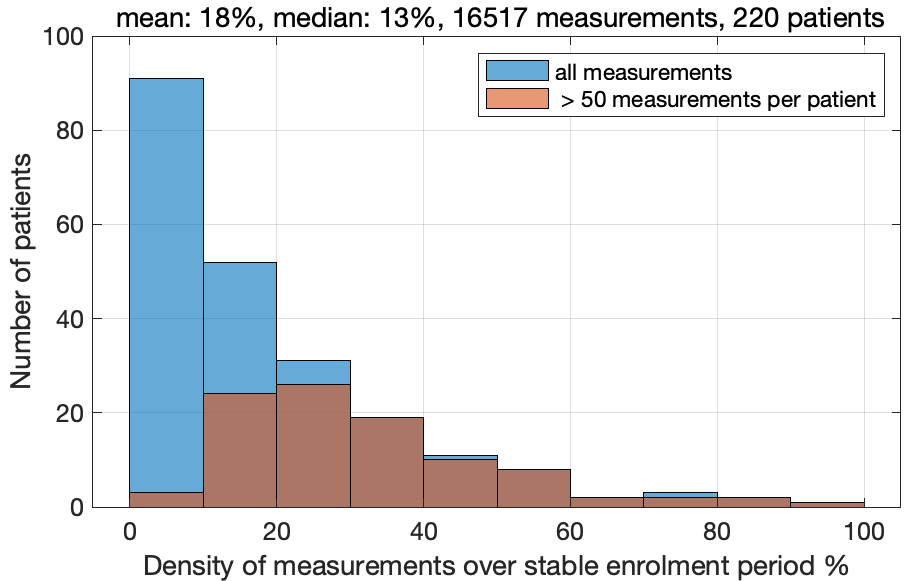
\includegraphics[width=65mm]{images/patientCommitmentFEV1stable.png}
    \caption{Patient commitment to FEV1 recording}
    \label{fig:commitment}
\end{figure}

\subsection{FEV1 variability}
Figure \ref{fig:variability} summarises a set of statistics, for (window size, threshold) pairs describing the residuals' sample, which can be taken as estimates of the variability. All models use over 66\% of patients and over 74\% of all stable measurements available. This strengthens the constraints \textbf{C2} and \textbf{C3}. 

\begin{figure}[!h]
    \centering
    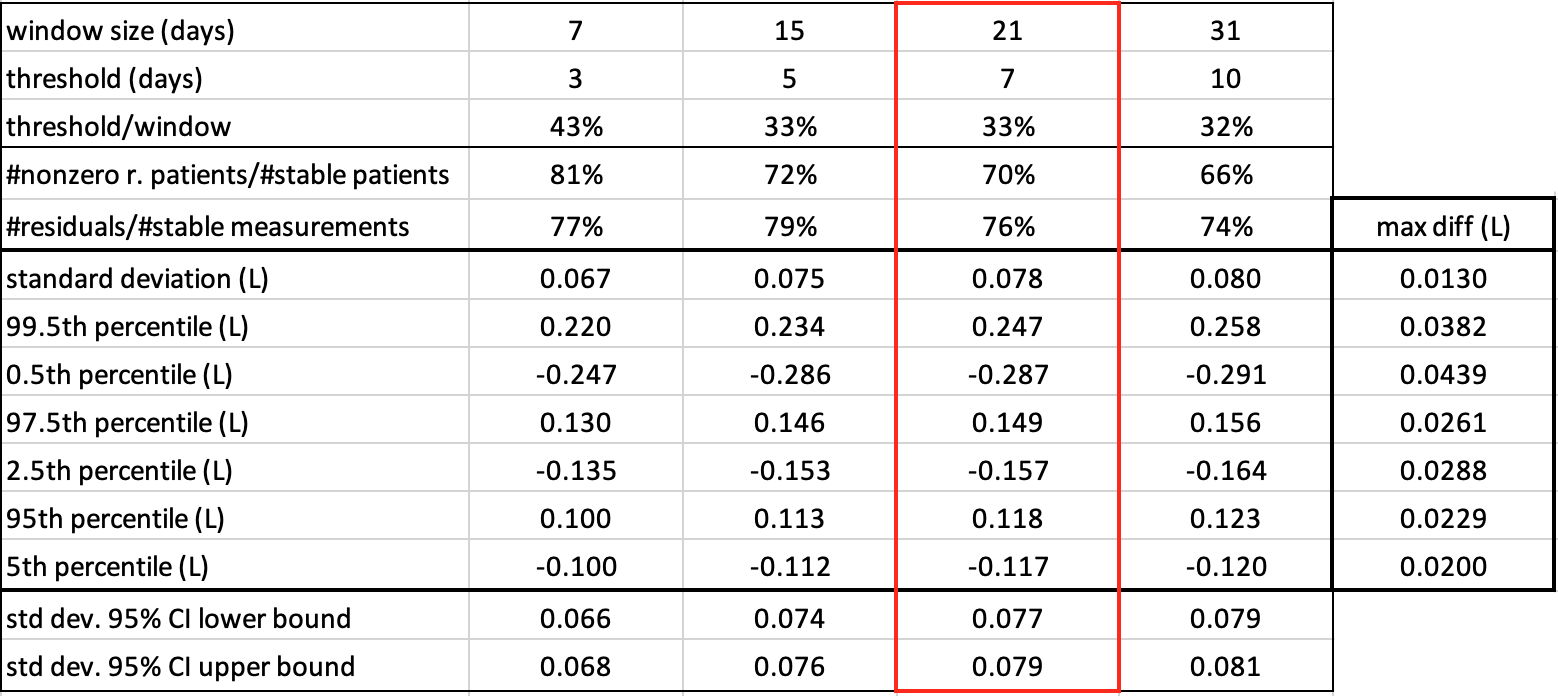
\includegraphics[width=140mm]{images/variabilitytable.png}
    \caption{Model results for different parametrisation}
    \label{fig:variability}
\end{figure}

The sensitivity of the statistics with respect to the choice of the parameters is of the order of 10 mL, which is low since one would expect significant variations in volume to be of the order of 100 mL. Nevertheless, the parametrisation (21,7) is the most conservative to ensure all constraints apply, an example is given in figure \ref{fig:fev1profile}. In fact, with (7,3) and (15,5) the minimum smoothing scale is of 3 and 5 days which is too close to the time-scale of the variations of noise (\textbf{C2}). (31,10) could be the best alternative to (21,7) but 21 days of smoothing window already a conservative choice to ensure that all noise has been removed (\textbf{C1}). 

The 99.5th precentiles is located over three sigma deviations, the 97.5th percentile at 2 sigma, and the 95th percentile at 1.5 sigma. Whereas the 2.5th-97.5th and 5th-95th percentiles ranges are stable, the absolute value of the residuals' are unbalanced nearby the 0.5th percentile compared to the 99.5th percentile. This suggests that the 0.5th-0.95th already contain outliers. The most reasonable statistics to estimate the variability are therefore the 2.5th-97.5th range, or two sigma, leading to a variability of 306 mL, respectively 312 mL. Hence, 310 mL can be set as a clear ground rule for clinicians.

\begin{figure}[!h]
    \centering
    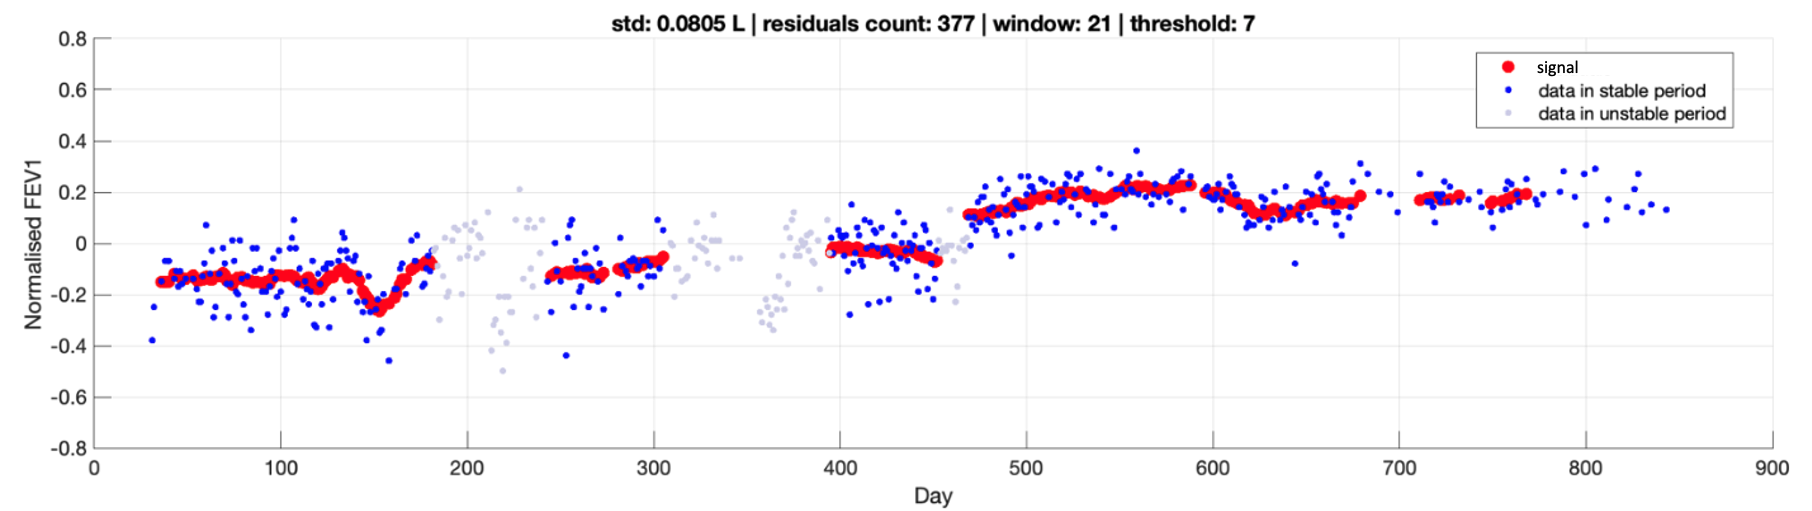
\includegraphics[width=150mm]{images/fevMovingAvg_patient103_w21_t7.png}
    \caption{Patient FEV1 measurements profile with the residuals from the (21,7) moving mean filter}
    \label{fig:fev1profile}
\end{figure}
\subsection{Categorisation of patients' variability}
Based on the standard deviation, the dispersion of the variability among patients is extremely high. The boxplot figure \ref{fig:fev1boxplot} shows that the standard deviation of the patients’ residuals ranges between 46 mL (25th percentile) and 107 mL (75\% percentile), which is more than the double. Defining the variability as two standard deviation, the variability would range in [184; 428] mL. From observations of the FEV1 profiles, the residuals’ standard deviation is an excellent method to segment patients between high, medium and low FEV1 variabilities.

\begin{figure}[!h]
    \centering
    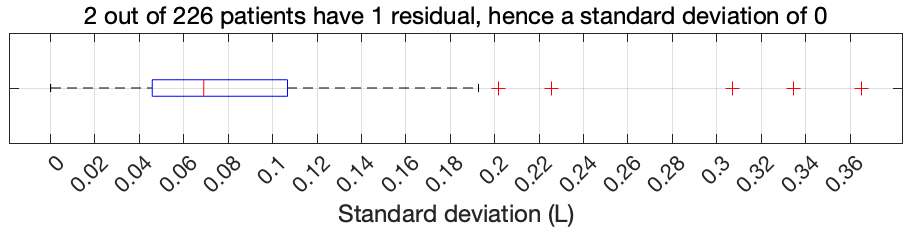
\includegraphics[width=90mm]{images/fev1boxplot.png}
    \caption{Boxplot of the patients' standard deviation in FEV1 measurements}
    \label{fig:fev1boxplot}
\end{figure}

\subsection{Relation with predicted FEV1\%}
Clinically, it would be interesting to know if one could differentiate patients' lung function based on their variability. FEV1 in percent predicted was used to evaluate patients' mean FEV1 on the same reference scale based on their height. However, the Pearson correlation coefficient of 0.129 shows insignificant correlation (p-value = 0.222 \ref{fig:correlation}). 

\begin{figure}[!h]
    \centering
    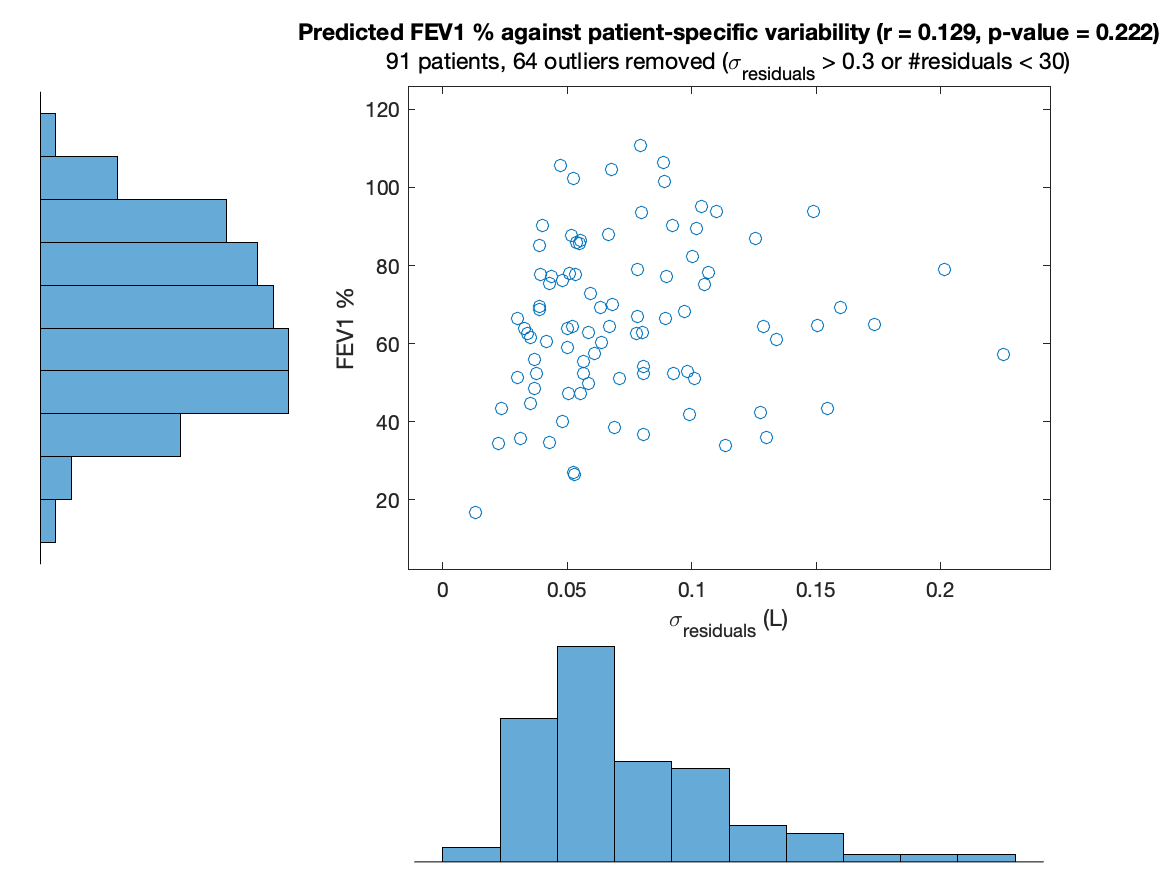
\includegraphics[width=100mm]{images/fevModelBasedAnalysis_variabilityvsFEV1.png}
    \caption{Correlation of variability and lung health}
    \label{fig:correlation}
\end{figure}

\subsection{Effect of CFTR modulator therapies: homoscedasticity test} \label{sec:hptests}
As explained in the introduction, CFTR modulators are transforming life of cystic fibrosis patients. Since 69\% of our participants were prescribed Triple Therapy, and 47\% Symkevi (figure \ref{fig:breathestats}), the data set was deemed sufficiently rich in to analyse the effect of CFTR modulators on the FEV1 variability during stable period. Three homoscedasticity were performed tests on 1) "prior Symkevi" - "during Triple Therapy", 2) "during Symkevi" - "during Triple Therapy", 3) "prior Symkevi" - "during Symkevi", to see if treatments had a significant effect on the reduction in variability. To do that, 5 more patients were removed whose residual's standard deviation were far outlying (> 0.19, figure \ref{fig:fev1boxplot}), in addition to the three from the model parametrisation. 76 patients that were chronologically prescribed Symkevi and then Triple Therapy, were selected. Note that any data after a Triple Therapy stop, this concerned 6 individuals (table \ref{tab:cftrmodulators}), were removed. This data was partitioned into three groups: A) measurements performed prior Symkevi, i.e. no therapy, B) during Symkevi, and C) during Triple Therapy. The Q-Q plot showed that the samples had a Student t-location-scale distribution (figure \ref{fig:qqplot}). Considering samples of over 1000 elements, the few outliers (<20) are indeed negligible. The Student distribution is a two tailed distribution with tails heavier than the normal distribution, and it is very close to the Cauchy distribution for small degrees of freedom and large sample sizes. Since this is the case ($\nu$=\{3;4\}), the best test is therefore the Levene's test with 10\% trimmed mean as defined in \ref{sec:homoscedasticity} as well as an right-tail F-test to maximise robustness. 

\begin{figure}[!h]
    \centering
    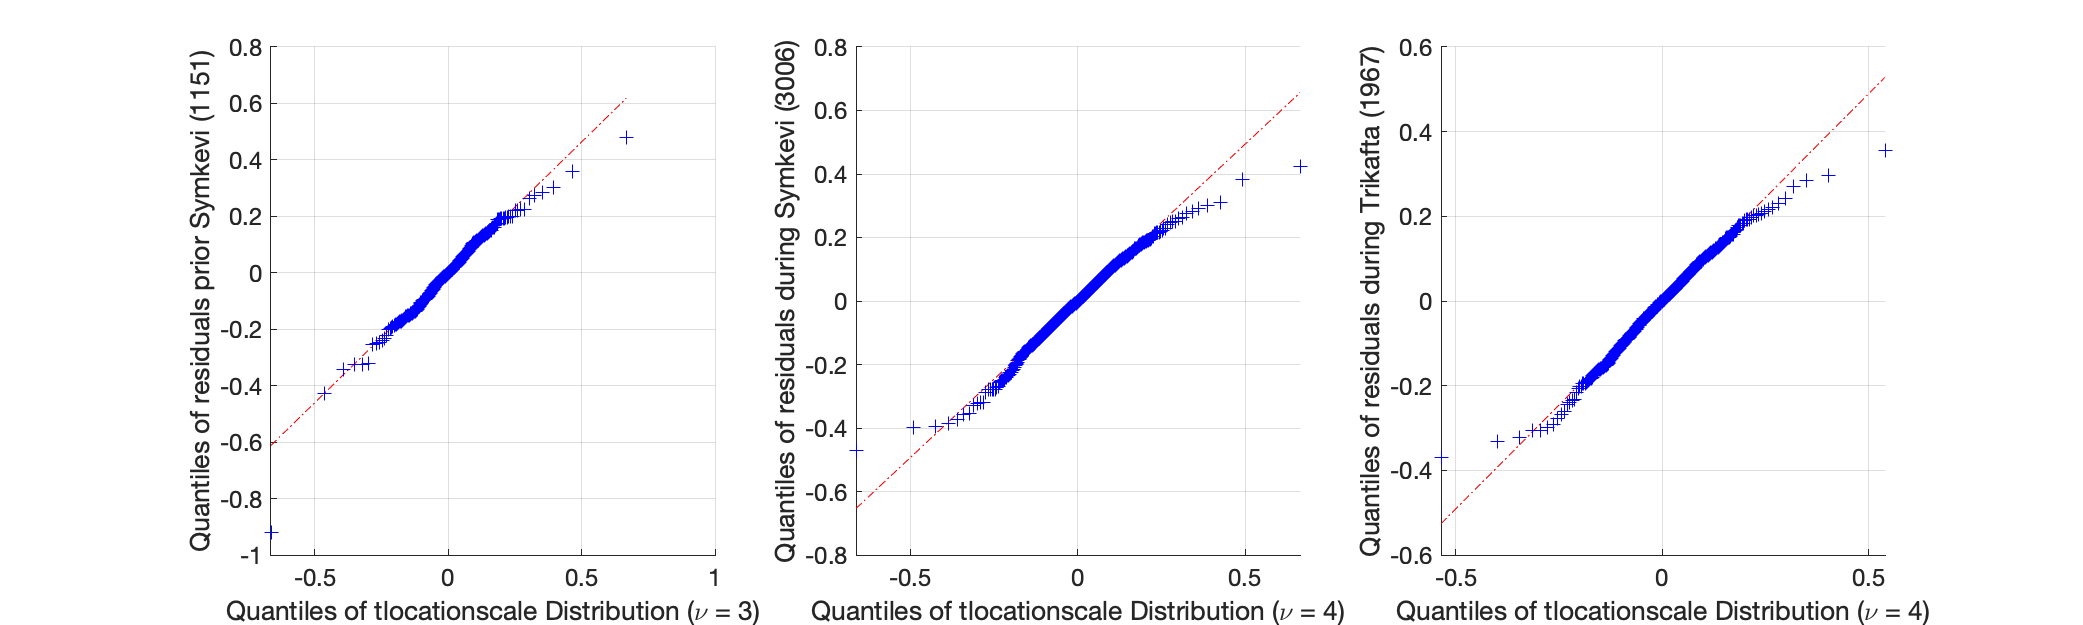
\includegraphics[width=150mm]{images/fevModelBasedAnalysis_qqplot_none_smkv_trpl.png}
    \caption{Q-Q plot of the three groups}
    \label{fig:qqplot}
\end{figure}

The tests 1, 2, 3 summarised on figure \ref{fig:hptests} showed a significant reduction, with below 3\% significance threshold, in the FEV1 variability after the start of Triple Therapy over  Symkevi (7\% reduction in standard deviation) and the start of Triple Therapy over no therapy (17\% reduction in standard deviation). However, the variability reduction was not significant after Symkevi start over no therapy. 

\begin{figure}[!h]
    \centering
    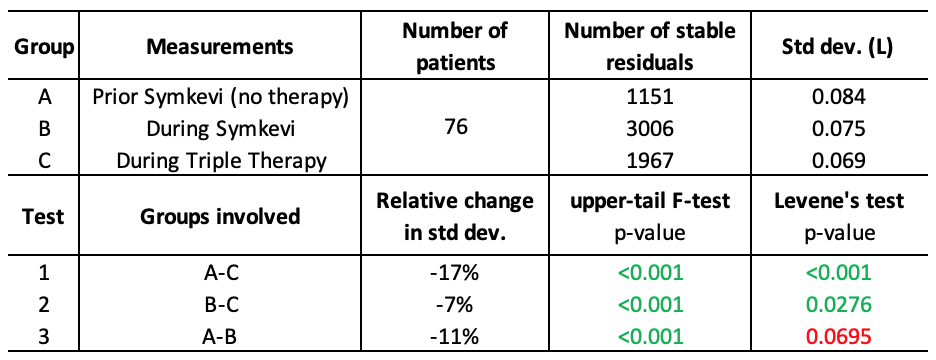
\includegraphics[width=100mm]{images/tests.png}
    \caption{Tests 1, 2, 3 on equality of variance}
    \label{fig:hptests}
\end{figure}

Two additional tests where performed with a similar setting: 4) "anything before Triple Therapy" - "during Triple Therapy", and 5) "anything before Symkevi" (except Triple Therapy) - "during Symkevi". Q-Q plots were extremely close to \ref{fig:qqplot}. Powerful statistical significance for the start of Triple Therapy over any CFTR modulator history (p<0.001) was obtained, but not for Symkevi against prior therapies (figure \ref{fig:hptests2}.

\begin{figure}[!h]
    \centering
    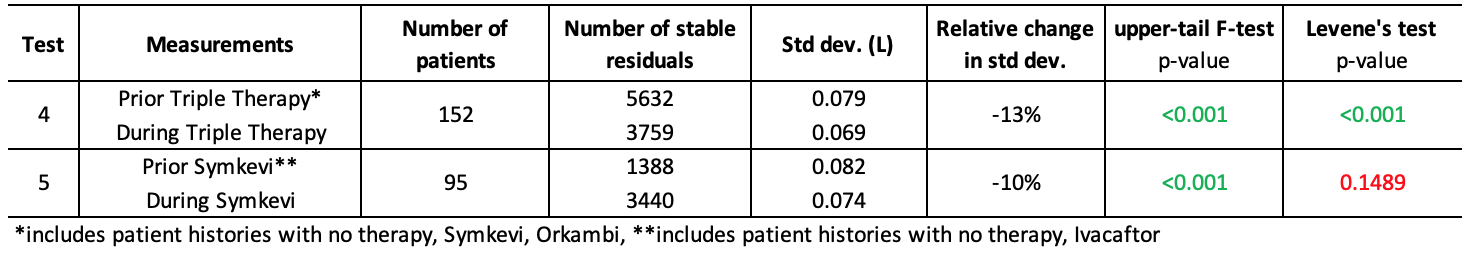
\includegraphics[width=150mm]{images/hptests2.png}
    \caption{Tests 4, 5 on equality of variance}
    \label{fig:hptests2}
\end{figure}


\section{Discussion}
A model was created to estimate the FEV1 measurements variability based on the residual's of a bi-parameter moving mean filter. Based on 150 patients and 12550 measurements, the variability of FEV1 measurements was estimated to 310 mL, using the span of the 2.5, 97.5th percentile in figure \ref{fig:variability}. This results is more conservative than for the standard deviation, the gold standard for measuring variability. Also, it verifies the work from Cooper et al., 1990 who estimated it to 260 mL, using the 95th percentile (this would give 230 mL in this study \ref{fig:variability}), with a much smaller data set of 28 patients and 9 measurements each \cite{cooper_1990}.

However, \textbf{the variability is extremely diverse among patients}, with a median at 276 mL and large interquartile range deviations of -92 mL (-33\%) and +152 mL (+55\%). Consequently, any precise study of FEV1 signal should not use a global approximation for the FEV1 variability to distinguish signal from noise, but rather a much more precise patient-specific value, which can be selected as the patient's standard deviation of the residuals. Additionally, this variability could be explained with predicted FEV1\% (Pearson correlation coefficient r=0.129). 

Eventually, it was demonstrated powerfully and robustly that \textbf{the start of Triple Therapy led to significant mitigation of the variability} in FEV1 over \textit{any} previous CFTR modulator therapy history available, with six hyptohesis tests (with p<0.001 for 5 of them). Also important, statistical significance for reduction in FEV1 variability for the start of Symkevi over any previous CFTR modulator therapy history available was not shown.

\subsubsection{Model limitations}
After removing unstable measures, the dataset can still contain day-to-day signal variations because 1) some CFTR modulator events may not have been recorded by hospitals, and 2) stable periods of FEV1 measurements can contain unstable measurements.  Nonlinearities in the measurement device output can modify the scale of signal and noise for each measurement, thus perturbing the results. The extent to those limitations are unknown and standard for a clinical study involving manually reported values and measurements.